\documentclass[
%% TIKZ_CLASSOPTION %%
tikz
]{standalone}
\usepackage{amsmath}
\usetikzlibrary{matrix}
%% EXTRA_TIKZ_PREAMBLE_CODE %%
\begin{document}
%% TIKZ_CODE %%
\usetikzlibrary{arrows}
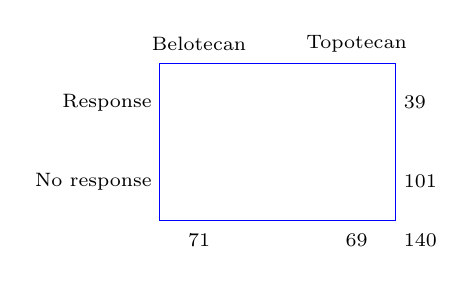
\begin{tikzpicture}[scale=1]
\scriptsize
\thicklines
% rectangle
\draw[blue] (0,0) rectangle (3,2);
% Marginal counts
\path (0.5,2.25) node[centered]{Belotecan};\path (2.5,2.25) node[centered]{Topotecan};
\path (0,1.5) node[left]{Response};\path (0,.5) node[left]{No response};
\path (3,1.5) node[right]{39};\path (3,.5) node[right]{101};
\path (0.5,-.25) node[centered]{71};\path (2.5,-.25) node[centered]{69};\path (3,-.25) node[right]{140};
\end{tikzpicture}
\end{document}
